\documentclass[oneside,a4paper,12pt]{article}
\usepackage{graphicx}
\usepackage{amsmath}
\usepackage{listings}
\graphicspath{{~/templates/}, {../images/}}

\makeindex
\begin{document}
	\begin{titlepage}
		\includegraphics[width=4cm]{logopopo.png}
		\hspace*{\fill}
		\includegraphics[width=6cm]{logouniv.png}
		
		\begin{center}
			\vspace{1cm}
			\textbf{TP Support de Transmission}\\
			\textbf{Mélageur à diode}\\
			\vspace{1cm}
			\textbf{Maxence LAURENT, Thibault VOLLERIN, Maxence NEUS}\\
			\vspace{3cm}
			%\includegraphics[width=13cm]{titlepage.png}\\
			\vspace{\fill}
			\textbf{Mars 2022}\\
		\end{center}
	\end{titlepage}
	
	\tableofcontents
	
	\vspace{5cm}
	
	\begin{abstract}
	
 	\end{abstract}

	\newpage

	\section{Préparation}
	
	\newpage

	\section{Manipulations}

	\subsection{Etalonage}


	
	\subsection{Isolations}

	\begin{figure}[h]
		\centering
		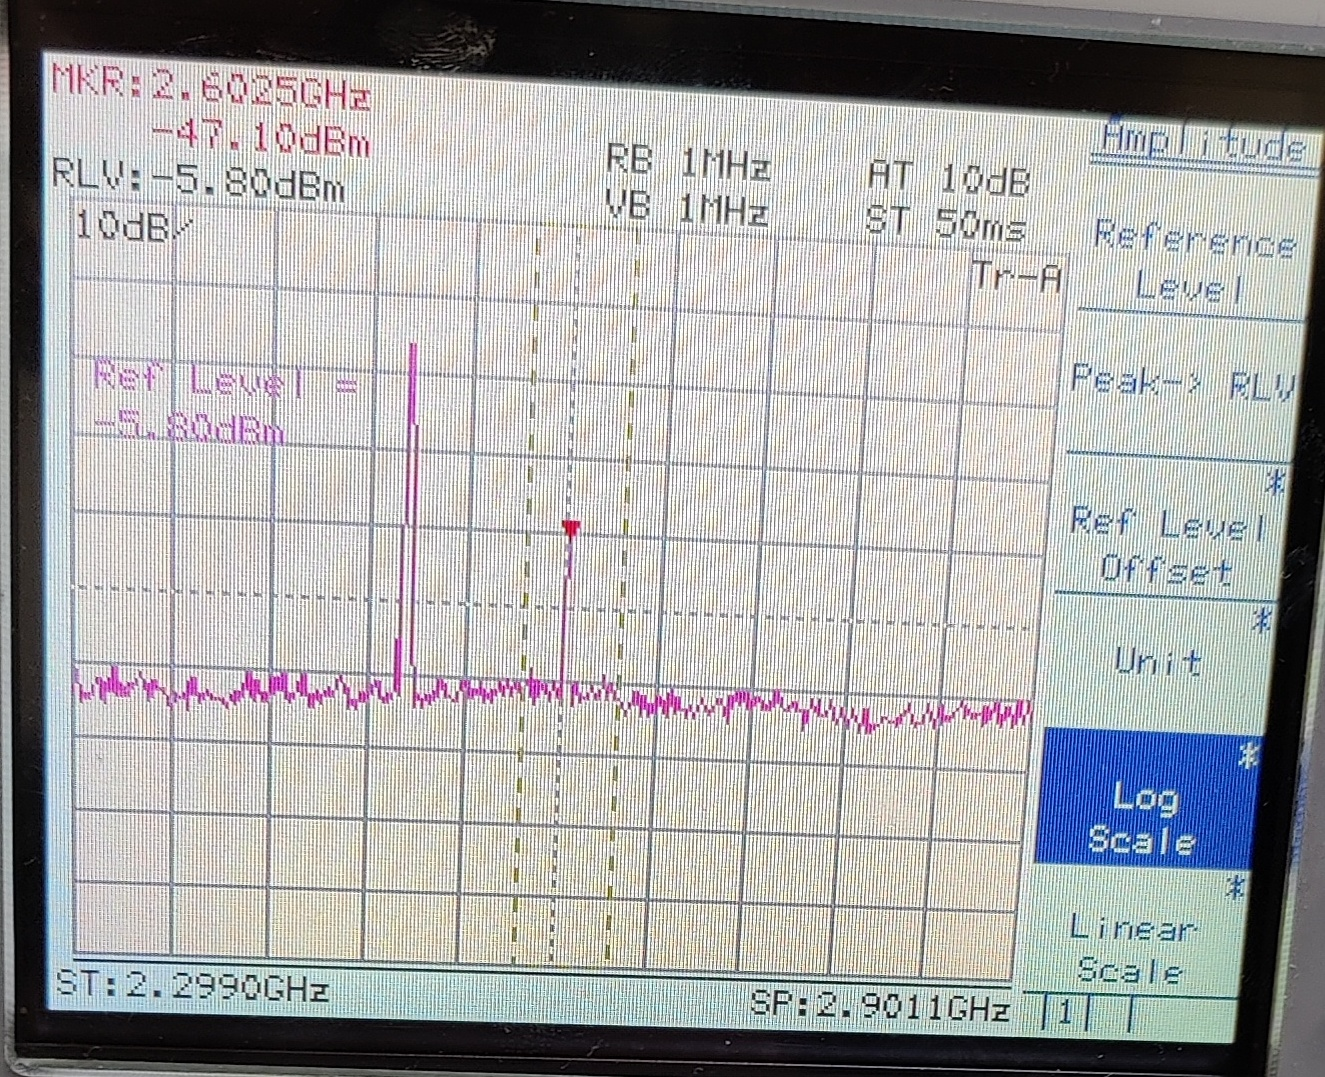
\includegraphics[width=8cm]{manip1.jpg}	
		\caption{Raies en voie IF}
	\end{figure}

	On a mesuré les puissances des raies :
	\[ P_{OL}(IF) = -22dBm \]
	\[ P_{RF}(IF) = -47dBm \]

	Isolations :
	\[ I_{RF_IF} = P_{RF}(RF) - P_{RF}(IF) = (-20 dBm) - (-47 dBm) \]
	\[ I_{RF_IF} = 27 dB \]

	\[ I_{OL_IF} = P_{OL}(OL) - P_{OL}(IF) = (7 dBm) - (-22 dBm) \]
	\[ I_{OL_IF} = 29 dB \]

	\subsection{Pertes de conversion}

	\begin{figure}[h]
		\centering
		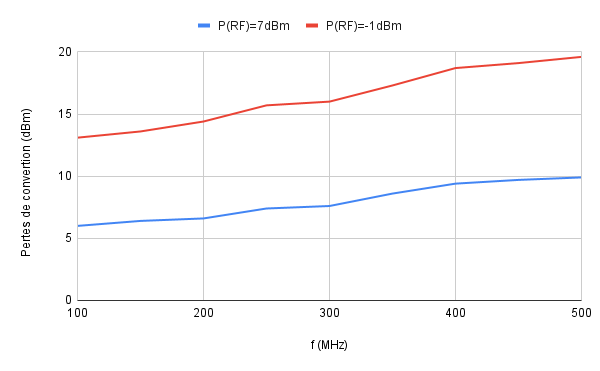
\includegraphics[width=10cm]{pertesfIF.png}	
		\caption{Pertes de convertions en fonction de $f_{IF}$}
	\end{figure}
	
	\begin{figure}[h]
		\centering
		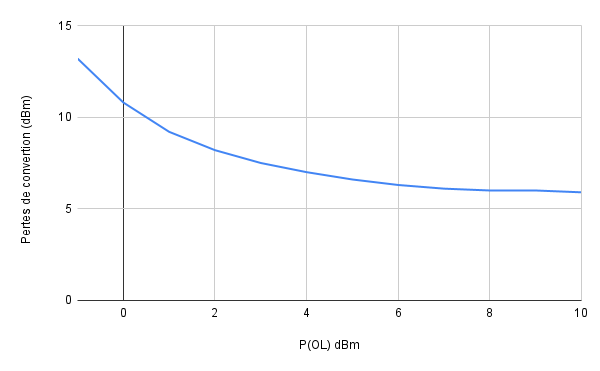
\includegraphics[width=10cm]{manip2.png}	
		\caption{Pertes de convertions en fonction de $P_{OL}$}
	\end{figure}

	\begin{figure}[h]
		\centering
		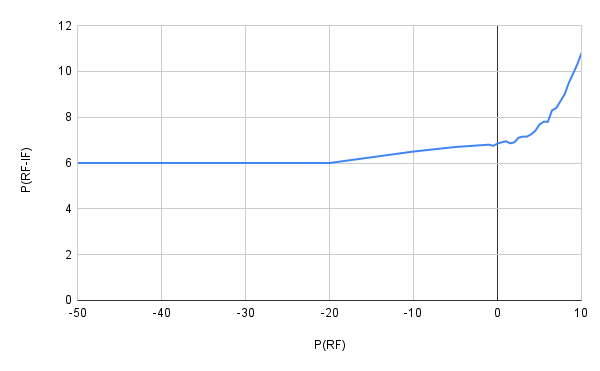
\includegraphics[width=10cm]{ptCompression.png}	
		\caption{Pertes de convertions en fonction de $P_{RF}$}
	\end{figure}

	\newpage
	\section{Conclusion}

\end{document}
